\documentclass[english,onecolumn]{IEEEtran}

\usepackage[T1]{fontenc}
\usepackage[latin9]{luainputenc}
\usepackage[letterpaper]{geometry}
\geometry{verbose}
\usepackage{babel}
\usepackage{extarrows}
\usepackage[colorlinks]{hyperref}
\usepackage{listings}
\usepackage{color,xcolor}
\usepackage{graphicx}
\usepackage{subfigure} 
\usepackage{amsthm,amssymb,amsfonts}
\usepackage{textcomp}
\usepackage{bm}
\usepackage{booktabs}

\providecommand{\U}[1]{\protect\rule{.1in}{.1in}}
\topmargin            -18.0mm
\textheight           226.0mm
\oddsidemargin      -4.0mm
\textwidth            166.0mm
\def\baselinestretch{1.5}

\DeclareMathAlphabet\mathbfcal{OMS}{cmsy}{b}{n}
\newcommand{\Ab}{\mathbf{A}}
\newcommand{\Bb}{\mathbf{B}}
\newcommand{\Ub}{\mathbf{U}}
\newcommand{\Vb}{\mathbf{V}}
\newcommand{\ub}{\mathbf{u}}
\newcommand{\vb}{\mathbf{v}}
\newcommand{\Ucal}{\mathbfcal{U}}
\newcommand{\Wcal}{\mathbfcal{W}}
\newcommand{\Vcal}{\mathbfcal{V}}
\newcommand{\Xcal}{\mathbfcal{X}}
\newcommand{\Ycal}{\mathbfcal{Y}}
\newcommand{\Rbb}{\mathbb{R}}

\begin{document}

\begin{center}
	\textbf{\LARGE{SI114H-Computational Science and Engineering, 2025 Spring}}\\
	{\Large Homework Set \#2}\\
\par\end{center}

\noindent
\rule{\linewidth}{0.4pt}
{\bf Requirements:}
\begin{enumerate}
	\item Deadline: {\bf \textcolor{red}{11pm, 12 May 2025}}. %Homework\#2 only contains the programming part.

	\item About your codes:
	\begin{enumerate}
	    \item Make sure that your codes can run and are consistent with your results.
	    \item Attach a {\textcolor{blue}{Readme.txt}} file to clearly identify the function of each file.
	\end{enumerate}

 \item You need to compress three files \textbf{code} (Only accept MATLAB language), \textbf{readme} (Add supplementary explanations to the code), and \textbf{PDF} (Show your results) into one file, name this file as \textcolor{blue}{student ID + your name} and send it to the blackboard system.

\end{enumerate}
\rule{\linewidth}{0.4pt}



\noindent\textbf{Problem 1}. \textcolor{red}{(100 points)} \par
Consider the following problem
\begin{equation}
    \begin{cases}
    -\frac{d}{dx}[C(x)\frac{du}{dx}] = 1 \ , \ 0<x<1,\\
    u(0)=u(1)=0,
    \end{cases}
    \label{problem}
\end{equation}\\
where \begin{equation}
    C(x)=\begin{cases}
        1  \ ,\  0<x<\frac{1}{2},\\
        \frac{1}{2} \ , \  \frac{1}{2}\leq x<1.
    \end{cases}
\end{equation}

Program the finite element method (FEM) to solve the problem \eqref{problem}. Denote the number of elements as $n$. Exhibit the corresponding solutions with $n = 4, 8, 1000$ in your report. 
\begin{enumerate}
    \item \textcolor{red}{(30 points)} Give the stiffness matrix $\boldsymbol{A}$, vector $\mathbf{f}$ and solution $\mathbf{u}$ for $n = 4$.
    \item \textcolor{red}{(60 points)} Give the value of $u(\frac{1}{4})$ and $u(\frac{3}{4})$ for $n = 4, 8, 1000$.
    \item \textcolor{red}{(10 points)} Plot the solutions in one figure for $n = 4, 8, 1000$.
\end{enumerate} 

Solution: \\

\begin{enumerate}
    \item  The stiffness matrix $\boldsymbol{A}$, vector $\mathbf{f}$ and solution $\mathbf{u}$ for $n = 4$ are as follows:
    \begin{equation}
        \boldsymbol{A} = \begin{bmatrix}
            4   & -4  &   0  &   0  &   0\\
            -4   &  8   & -4  &   0  &   0\\
            0  &  -4  &   6  &  -2  &   0\\
            0  &   0  &  -2   &  4  &  -2\\
            0   &  0  &   0  &  -2  &  2\\
        \end{bmatrix}, \quad
        \\
        \mathbf{f} = \begin{bmatrix}
            0.1250\\
            0.2500\\
            0.2500\\
            0.2500\\
            0.1250\\
        \end{bmatrix}, \quad
        \\
        \mathbf{u} = \begin{bmatrix}
            0\\
            0.1146\\
            0.1667\\
            0.1458\\
            0\\
        \end{bmatrix}.
    \end{equation}
    \item The values of $u(\frac{1}{4})$ and $u(\frac{3}{4})$ for $n = 4, 8, 1000$ are as follows:\\
    
    Results for u(1/4) and u(3/4):\\
    n = 4: u(1/4) = 0.114583, u(3/4) = 0.145833\\
    n = 8: u(1/4) = 0.114583, u(3/4) = 0.145833\\
    n = 1000: u(1/4) = 0.114583, u(3/4) = 0.145833\\
    This is a known property: for a 1D problem $-u^{''} =f $ with f constant, linear elements give exact nodal values. If f is piecewise constant and discontinuities are nodes, it's also exact. \\
    \item The plot of the solutions for $n = 4, 8, 1000$ is shown below:
    \begin{figure}[h]
        \centering
        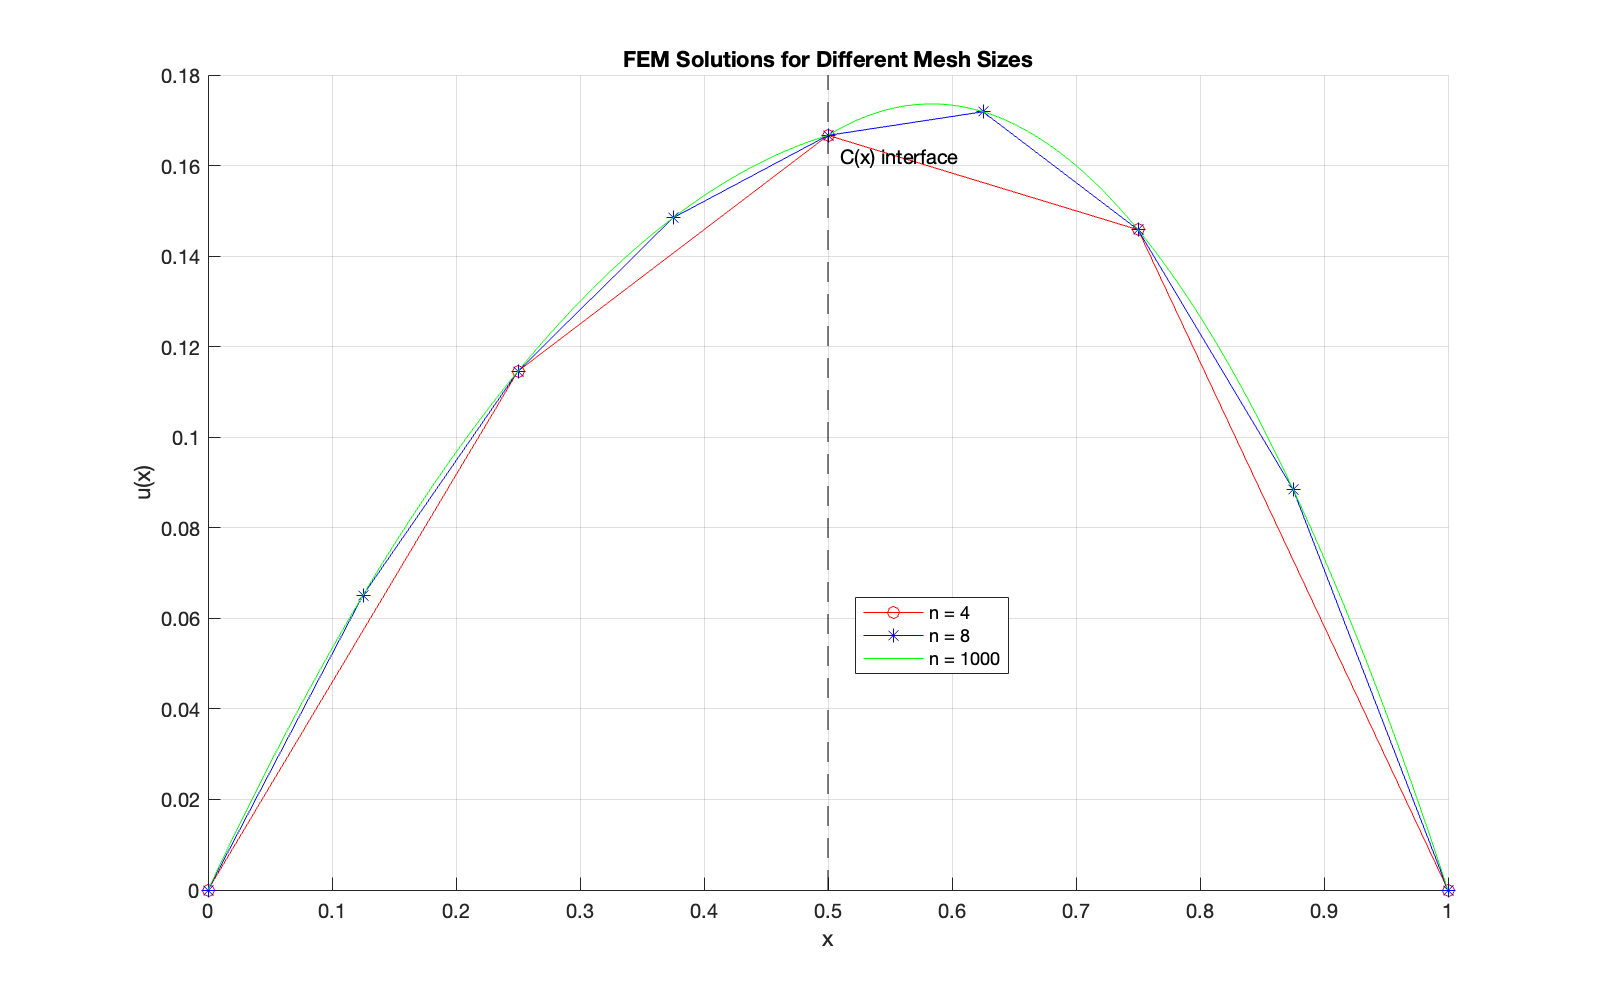
\includegraphics[width=0.8\textwidth]{p3.png}
        \caption{Plot of the solutions for $n = 4, 8, 1000$}
        \label{fig:solution_plot}
    \end{figure}
\end{enumerate}
\end{document}
